\documentclass[review]{elsarticle}

\usepackage{lineno,hyperref}
\usepackage{rotating}
\usepackage{algpseudocode,algorithm}
\usepackage{hyperref}

\graphicspath{ {./images/} }

\modulolinenumbers[5]

\journal{Future Generation Computer Systems}
\begin{document}

\begin{frontmatter}

\title{An Event-based Architecture for Multi-population Optimization Algorithms}

\author[itt]{Mario Garc\'ia Valdez}\corref{mycorrespondingauthor}
\cortext[mycorrespondingauthor]{Corresponding author}
\ead{mario@tectijuana.edu.mx}

\author[granada]{Juan J. Merelo Guerv\'os}
\ead{jmerelo@geneura.ugr.es}

\address[itt]{Department of Graduate Studies, Instituto Tecnol\'ogico de Tijuana, Tijuana BC, Mexico}
\address[granada]{Universidad de Granada, Granada, Spain}

\begin{abstract} 
Splitting a population into multiple instances is a technique that has been used extensively in
recent years to improve the performance of nature-inspired optimization
algorithms. Work on several populations can be done in parallel, and
also asynchronously, which can be leveraged to create scalable
implementations based on, among other methods, distributed, multi-threaded, parallel, and cloud-based computing. 
% I have rephrased all this. Please check it out - JJ
The design of these cloud-native, distributed, multi-population
algorithms is not a trivial task. Coming from monolithic
(single-instance) solutions, adaptations at several levels, from the
algorithmic to the functional, must be made to leverage
the scalability, elasticity, fault-tolerance, reproducibility, and
cost-effectiveness of cloud systems while, at the same time,
conserving the intended functionality. Instead of an evolutive
approach, in this paper we propose to create from scratch a
cloud-native optimization framework that is able to include multiple
algorithms and use few parameters to work. This solution goes beyond
current state of the art via a framework that is able to support
different algorithms at the same time, work asynchronously, and also
be easily deployable to any cloud platform. We evaluate the
performance and scalability of this solution, together with the effect
other design parameters had on the 
performance, in particular, the number and the size of populations
with respect to problem size. The architecture and the implemented platform is an excellent
alternative for running locally or in the cloud, thus proving that cloud-native
bioinspired algorithms perform better in their "natural" environment than other
kinds of algorithms, and setting a new baseline for scaling and
performance in the cloud.
% Still a big longish. We need another iteration to reduce it - JJ
\end{abstract}

\begin{keyword}
Multi-population \sep Nature-inspired algorithm \sep Parallel Genetic Algorithms \sep Cloud-Computing
\sep Event-driven architecture 
\end{keyword}

\end{frontmatter}

\linenumbers

\section{Introduction}

In the last decades, nature-inspired optimization algorithms have been succesfully
applied to solve complex real-world problems \cite{yang2014nature}. Algorithms
inspired by natural processes include evolutionary algorithms (EAs)
\cite{back1996evolutionary} and swarm intelligence (SI) \cite{kennedy2006swarm},
among others. These population-based algorithms share the common characteristic
of using an initial set of random candidate solutions that are later used to
generate a new set of candidates, using a nature-inspired heuristic. Popular EAs
are Genetic Algorithms (GAs) \cite{holland1992adaptation,eiben2003genetic}, 
Genetic Programming (GP) \cite{back1996evolutionary}, Grey Wolf Optimization
(GWO) \cite{mirjalili2014grey} and Differential Evolution (DE) \cite{karabouga2004simple},
while examples of (SI) \cite{kennedy2006swarm} are particle swarm
optimization (PSO) \cite{clerc2010particle} and ant colony algorithms (ACO) \cite{dorigo1999ant}.

Population-based algorithms are intrinsically parallel, and can be implemented to run asynchronously.
The fitness of each individual can be evaluated independently of 
others, and similarly, each population could evolve in isolation. Since 
earlier works, researchers have been proposing some form of parallelization
\cite{muhlenbein1988evolution} to increase the scalability of these algorithms.
The island model was one of the first techniques proposed for parallelization,
which lead to an increased performance \cite{gorges1990explicit,grosso1985computer}. 
The concept was to divide a large population into communicated subpopulations. 
Since then, other population-based algorithms have adopted the concept, 
and researchers have found additional benefits
besides the execution speed; these include avoiding a premature convergence and
maintaining the diversity of the global population \cite{li2015multi}. Researchers use the term
multi-population based methods when generally referring to techniques using
subpopulations as part of their optimization strategy. % Some comment about asynchrony would be in order - JJ
% Comments below - Mario
Moreover, parallel implementations can run in two ways: synchronous and
asynchronous. When operations run in parallel but must maintain synchronism with
the other operations,  all operations need to finish to continue to the next
step. For instance, in a  parent/worker model, the parent needs to wait for all
workers to finish their operations before moving to the next iteration.  In
contrast, in an asynchronous execution,  operations are not synchronized with
each other. Following the previous example, now the parent operation can
continue to the next iteration, even if a worker has not finished its work.  In
the literature, we can find many asynchronous algorithms
\cite{coleman89,baugh2003asynchronous}, reporting benefits in execution time,
and scalability. In the particular case of asynchronous and cloud-native
multi-population algorithms, recent works propose an asynchronous communication
through a central repository \cite{sofea:cec2012, JSON} or message queues
\cite{salza2019speed, guervos2018introducing}, in this work we follow this
practice.

The trend concerning the parallel execution multi-population algorithms go from
earlier hardware-based implementations using transputers
\cite{gorges1990explicit}, multi-threaded \cite{merelo2019scaling}, and
multi-core systems \cite{Serrano2008,lai2019adaptive}. % many citations here - JJ 
And recently the focus has been on exploiting a higher number of processing
units by using GPUs \cite{tan2015survey,li2007efficient}, or distributed
systems; techniques used to achieve this include web-based \cite{JSON},
map-reduce \cite{fazenda2012},  grid \cite{munawar2010design,Gonzalez09},
voluntary computing \cite{MilkyWay}, and cloud computing
\cite{GValdez2015,salza2019speed,valenzuela2015implementing,FlexGP}. % many references here too - JJ 
Cloud computing has become the standard way of running
enterprise applications, not only because of the convenience of the
pay-as-you-go model or the non-existent cost of administration, but also because
it offers a way of describing the infrastructure as part of the code, so that it
is much easier to reproduce results and this has been a boon for scientific
computing.  However,  cloud computing has also been evolving, going from simply
putting in the cloud old-style monolithic applications, that is, applications
built on a single stack of services that communicate by layers, to microservices
\cite{microservices} and serverless architectures \cite{varghese2018next,
Varghese2018849} that favor the parallel and asynchronous communication of
heterogeneous resources; in the process, a new process for designing {\em cloud
native applications} has been created, with brand new methodologies and
techniques \cite{Baldini2016287}. In these architectures, services or even
functions are seen as single processing points, departing from the monolithic
and even distributed paradigms, become a loosely coupled collection of {\em
stateless functions} \cite{malawski2017serverless}, that react to events and
only come into existence while they are doing some processing. % many references more here - JJ 
Systems developed with the patterns outlined above have the
properties of a reactive system \cite{boner2014reactive} and they are commonly
more flexible, loosely-coupled, and scalable. % Some properies and reference - Mario  
% Again, you have to justify the need for a reactive architecture and define it before this paragraph - JJ


When designing efficient multi-population algorithms, researchers need to
consider additional issues \cite{Ma2019}. These include the number and size of subpopulations,
the interaction between them, the search area of subpopulations, and the search
strategy and parametrization of each subpopulation. We must take into account
these high-level issues when designing a parallel architecture. Researchers 
and algorithm designers willing to  adapt to the cloud their
multi-population solutions face the additional challenges:
\begin{itemize}
    \item They need to change their current solutions to a reactive architecture in which processes
    communicate with each other by exchanging messages asynchronously and react
    to a continuous stream of data. One of the options is to consider
    sub-populations as messages to be modified asynchronously by functions. 

    \item To scale the system, when it is possible, they must use stateless functions for
    processing. 

    \item They need to establish a workflow of local development and prototyping while having the 
    option of deployment in a cloud provider. It is desirable to use modern development methodologies and technologies. 

    \item They must log experimental results and be able to replicate the experiments. 

    \item They must consider additional parameters that can affect the monetary cost or the performance of the
    execution — for instance, the format and size of messages, the number of
    worker processes and their capabilities.  
\end{itemize}

Taking these factors into account, in this work, we present EcoSwarm, % maybe a less generic name? - JJ
% agree - Mario
a multi-container Docker application that reactively processes isolated and
heterogeneous subpopulations. The platform uses the Docker Compose tool for
defining and running experiments as multi-container applications. 
% Docker compose is not really for production, more for development environments, 
% you have to justify this. Also, it does not handle scaling so need to justify it too - JJ
% justification: - Mario
We preferred the use of a container-based application for this prototype because
it is more suitable for development and replication without the need for
additional components. Nevertheless, the application is compatible with other
orchestration and deployment technologies if more scalabilty is needed. 
With additional configuration settings, applications can be deployed 
to a Docker Swarm or a Kubernetes system.  

Docker Container images host the stateless functions responsible for running 
a search strategy on subpopulations, these functions could also be ported
directly to a Function as a Service (FaaS) \cite{Roberts2016} implementation.
% Need to improve the next paragraph or maybe move it to another place - Mario
Researchers then define the configuration of services used by
a multi-population algorithm using a YAML file. Any researcher can deploy and
start all the services from this configuration file with a single command. Once
the services are up, multiple instances of an experiment can be sent to a queue
for their execution. The platform includes containerized services that are
compatible with other container orchestration technologies like Kubernetes and
Docker Swarm. The services included are a Redis Server used for the Message
Queue implementation and logging and an Experiment Controller implemented in
Python. Developers of sub-population processing functions have the freedom to
implement new population-based algorithms or operators in the language they
choose inside a container, as they only need to subscribe to a channel of the
Message Queue and have the ability to read the population and parameters as JSON  
file.

This paper extends our earlier publication on the topic
\cite{guervos2018introducing}, and we highlight the main contributions as
follows:

\begin{itemize}
    \item First, we present the design and implementation of a reactive 
    container-based application for the asynchronous execution of multi-population 
    algorithms. The source code and example container definitions are
    publicly available. % Not really a contribution. It's the mean to
                        % achieve the contribution - JJ
    \item Second, we propose a method for the deployment and execution of 
    multiple experiments by specifying the infrastructure as part of an 
    experiment definition in both local or cloud environments,
    facilitating the reproduction of experimental results. % Not clear
                                % what the contribution is. If this
                                % has been used for the first time in
                                % an EA environment, it should be
                                % stated that way. If not, it's also a
                                % mean to achieve the contribution - JJ
    \item Third, the application is compatible with the COCO benchmark 
    framework, allowing researchers to compare the performance of their 
    algorithms with other works. % Not really a contribution, but an
                                % implementation detail. Convenient,
                                % but does not advance the state of
                                % the art - JJ
    \item Lastly, we present an empirical study to validate the 
    applicability of our application,  measuring the execution time, 
    speedup, and a comparison between homogeneous and an ensemble of 
    multi-populations, using Genetic Algorithms (GAs) and Particle 
    Swarm Optimization (PSO) in a benchmark for the optimization of 
    continuous functions. % "Validate the applicability" falls short
                          % of being also a contribution. It must
                          % advance the state of the art, in which way
                          % does it advance? Speed (needs to be
                          % proved) Convenience (needs to be proved
                          % too) Scalability? (needs to be proved
                          % also). - JJ
\end{itemize}

The organization of the paper is as follows: First, in Section \ref{multi}, we present a
background of the fundamental issues of integrating nature-inspired optimization
and multi-population methods. Section \ref{soa} presents state of the art relevant to
our work. In Section \ref{method}, we present the proposed method and the container-based
application in Section \ref{docker} .  Section \ref{setup} describes
the design of the empirical evaluation we designed to assess the effectiveness
of the method, and in Section \ref{results}, we report and discuss the results. Finally, we
offer the conclusions of this paper and suggestions on future work in Section \ref{conclusions}.


\section{Multi-population methods} % Is this part of the state of the
\label{multi}
                                % art? - JJ
% This the Background for the design decisions, but I think is also needed
% to better understand the state of the art.

% Also, multipopulation design of what?x
Multi-population based methods divide the original population into
smaller subpopulations or islands, with every subpopulation carrying out the
algorithm independently, with synchronous or asynchronous communication with the
rest of the islands. % exemplify how this is done in different
                     % metaheuristics, especially those we will be
                     % using here - JJ
This relative isolation helps in maintaining an overall
diversity since each subpopulation will search in a particular area, at least
between communications. The recombination mentioned above (mixing) or migration
between subpopulations is needed to avoid a premature convergence of candidate
solutions since smaller populations are known to perform better for a given
problem than bigger populations. % Smaller populations converge
                                % prematurely or perform better? - JJ
However, it gives them the added advantage of
parallel operation. Additionally, and in some cases, multi-population algorithms
scale better than expected due to the interaction between the algorithm and the
parallelism of the operation \cite{ALBA20027}. % Need to clarify this
                                % and if it extends to Swarm
                                % algorithms too
                                % Also, is your objective to achieve this superlinear speedup? - JJ

However, in most cases, algorithms applied to each subpopulation are
homogeneous, or at any rate, the same variant of the algorithm. As long as this
parallel operation is not synchronous, other population-based algorithms, or, as
a matter of fact, any algorithm, could be easily integrated. That is why several
works based on multi-population are heterogeneous, integrating various
optimization algorithms, and often performing better than single-population or
homogeneous optimization algorithms \cite{wu2016differential,nseef2016adaptive}.

Heterogeneous algorithms add another degree of freedom to the problem of finding
the correct parameter settings for an algorithm; because some parameters affect
the accuracy of the solution and the convergence speed of the algorithms as they
tip the balance between exploration and exploitation of the search space. On the
other hand, current studies show that by having a high number of subpopulations
interacting in parallel, the effect of the individual parameters of each
subpopulation is compensated by those selected in other
subpopulations. % reference - JJ
In this
work, we will use random settings within a specific range as results have shown
this is a valid solution to this problem. % This should have been
                                % mentioned in the introduction - JJ

Some parameters, specially the population size, are
kept fixed in order to control more easily the execution of the algorithm. For
instance, by having the size of subpopulations fixed, it is easier to control
the number of evaluations and the communication costs, when the algorithm is in
operation. % And to keep them more or less synchronized, which can be
           % interesting, too... But this should go to the
           % introduction also - JJ

Combining multiple algorithms, with different parameters, interacting with each
other at the same time, can benefit from the strengths of each. For instance, a
genetic algorithm could find a promising global solution that is not optimal
while another algorithm, more suitable for a local search, finds the global
optimum. This approach has been followed extensively in recent years, with
success. % References - JJ
Moreover, there is a need for frameworks, architecture, and
implementation models that can allow researchers the development of new
parallel, asynchronous, heterogeneous, and parameter-free algorithms in a scalable way.  

\section{State of the Art} 
\label{soa}
% a lot of this has been done in the previous method... Maybe there's
% not that much to do - JJ
Hadoop 
    Comparison \cite{ferrucci2018using}
    Hadoop\cite{fazenda2012} 
    FlexGP \cite{FlexGP}, 
    elephant56 \cite{salza2016elephant56},

Pool
    SofEA \cite{merelo2012sofea,sofea:cec2012} , 
    EvoSpace \cite{garcia2015evospace},
Volunteer
    evospace-js \cite{garcia2017evospace}
Queue
    Containers \cite{valenzuela2015implementing} \cite{salza2016approach} 
    Seamless local and Cloud \cite{leclerc2016seamless}
    Serverless KafKEO \cite{guervos2018introducing}, 
    Docker Orchestation \cite{dziurzanski2020scalable,zhao2019cloud}
PSO 
    PSO AWS \cite{li2015parallel}

\section{Proposed Method} 
\label{method} 

In this section, we present the design
and a container-based implementation of the model we propose for the execution
of multi-population based algorithms. We follow the requirements outlined in
Section \ref{multi} and the general design principles of cloud-native
applications we have mentioned earlier. As a first step, we describe the general
architecture first, and then  every component in detail. 

The most elemental data structure used throughout the system is the subpopulation; and at a higher
level, we can view the system as a continuous stream of subpopulations
flowing
% We talk about "multi-population" elsewhere, including the
% abstract. We should unify terminology - JJ
% "multi-population" is the whole thing, a subpopulation is a member of that.
% "A multi-population has many subpopulations or should we call them just populations?"
% I will add a comment about this in the Multi-population section -
% Mario
% use the usual "multi-deme" terminology. A population has different
% sub-populations nad uses a multi-deme implementation - JJ
% Let's talk about it, I am using the Multi-population terminology 
% maybe multi-dem is more common in the EA community but not 
% much in the Swarm Intelligence side?  
% Any how, we decide and explain the difference so readers of both 
% camps are Ok with it. 
% I prefer the use of population and something like the global population - Mario

from one process to the other. By "continuous stream," we mean that ideally,
everything must happen asynchronously without components needing to wait for
others. In this kind of system, this streaming functionality is normally
implemented by using a message queue system. For instance, if one process needs
to communicate a subpopulation to another, it must pack the sub-population into
a message, and then send the message 
% I don't know if
                                % asynchronously applies here. It's
                                % simply sent - JJ 
                                % Meaning it does not wait for a
                                % respone, it continues doing other
                                % stuff - Mario
% That's rather "fire and forget". Or simply say it's sent without
% waiting for a response - JJ
% corrected - Mario
to the queuing system without waiting for a response; this
means that after the process pushes the message, it continues its execution
without waiting for a result. On the other end, the recipient subscribes to the
message queue by defining an event handler method that is going to be triggered when a
message is pushed to it. The two components at each end of the queue are
Producers that push messages to the queue and Consumers that pull them. This
pattern is an essential component of a reactive architecture and makes
it 
highly scalable; one of the reasons for this is the use of functions
that have no secondary effects or access global storage, that is,
stateless functions. These functions do not need to read, keep, or modify data outside of the method. If
Consumers are implemented using stateless functions, and thus, there is no difference
between having one or many copies of the same function pulling work from the queue all at the
same time, because no side effects, including unwanted resource
locking problems,  are going to result from this concurrency.
% This is important and we should probably mention that in the
% introduction - JJ 
Based on these general principles we define next the proposed model.


\begin{sidewaysfigure}
    \centering
    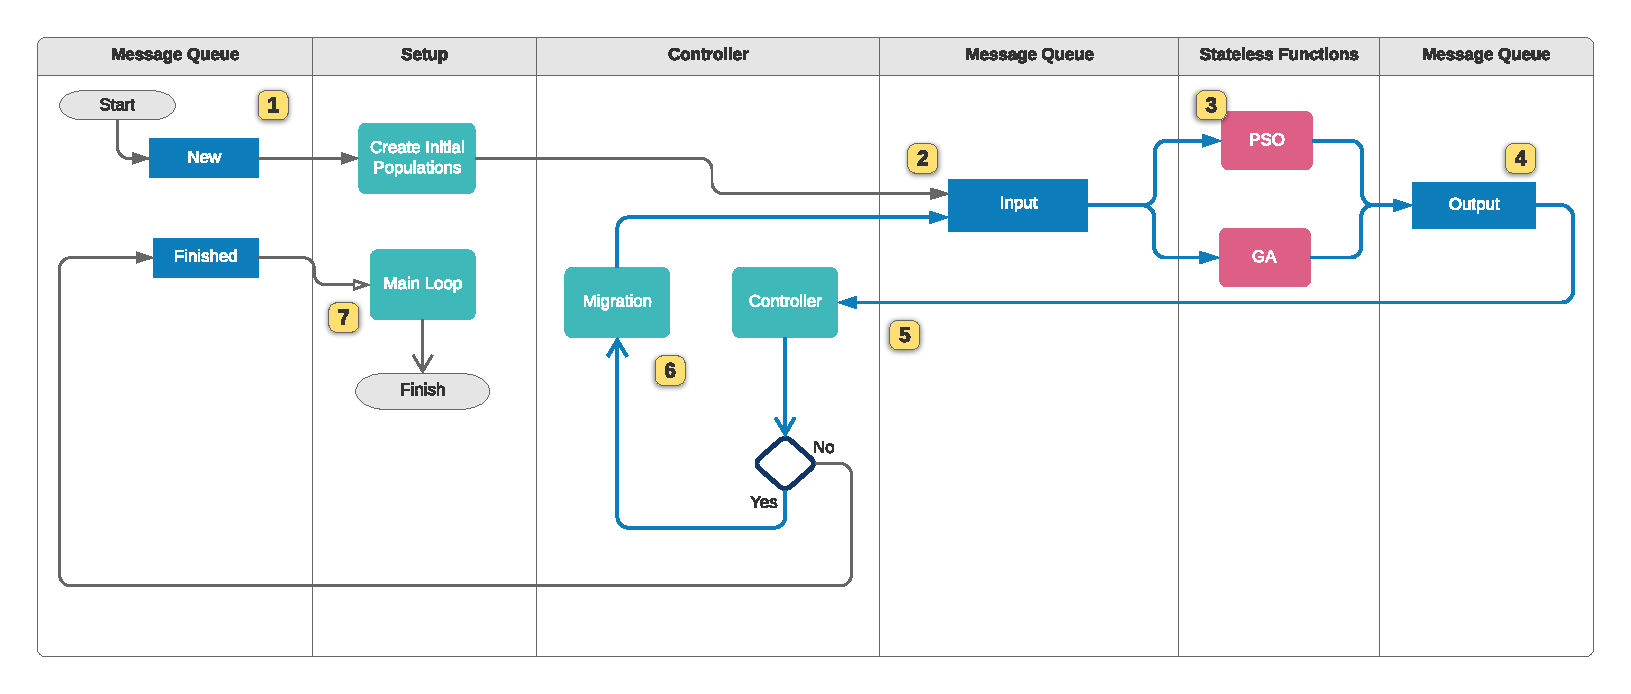
\includegraphics[width=\textwidth]{KafkEOsmall}
    \caption{The proposed general architecture, 
     showing each process in a swimlane, message-dataflow,
     message queues, and high-level tasks for each process.} 
    \label{fig:kafkEO}
\end{sidewaysfigure}

\subsection{Event Driven Model} 
\label{edm}
Based on a reactive architecture we proposed in a previous work
\cite{guervos2018introducing}, we now describe the general architecture shown in
Figure \ref{fig:kafkEO}. Again, we can explain the model using the analogy
of Producers and Consumers of messages. First, we can see that
there are two queues, one labeled Input, and the other one Output. In the diagram, 
push operations on a queue are represented by solid arrows connecting to the left side
of the box, and pull or pop operations as solid arrows leaving from the right side.
Also, the architecture has at least four processes indicated in the diagram as
swimlanes: First, the Setup process, responsible for the reading a configuration
file, and creating the initial subpopulations. Second, a Controller process,
responsible for the migration between subpopulations, and keeping track of the
iterations of the algorithm. The Message Queue process runs the Input and Output
queues. Finally, there is at least one Stateless Function process responsible
for running the isolated algorithms. In the example, two processes PSO and GA,
are shown. 

The algorithm starts with the Setup process pulling a configuration message from
the experiements queue, this is not shown in the diagram. The configuration messsage 
includes all the parameters needed to execute the algorithm, among other things,
the number of subpopulations, the number of individuals, and the number of iterations
of the algorithm. We give more details about the configuration data structure
in Section \ref{experiment_flow}. % Missing  % added 
Once the configuration is read, we can follow the path of 
messagess as follows:

\begin{enumerate}
\item In this step, the specified number of subpopulations is created acording to the 
parameters found in the configuration structure. The population at this moment is just
static data, including each individual inside. Each subpopulation includes a metadata
section where its algorithm and execution parameters are specified. For instance, 
for a GA, the mutation rate, type of crossover operator, and other values are indicated.

\item Each subpopulation is then pushed to the Input queue, so they can be consumed 
by Stateless functions responsible for the execution of the search.  % Why the caps in Stateless? - JJ  
% It refers to the swimlines in the diagram, maybe I should point it out  - Mario
% Added a comment above. - Mario

\item One or more Stateless functions are constantly pulling subpopulation messages
from the Input queue. Taking the population data and metadata as parameters, these 
functions are responsible for the actual execution of the optimization algorithm. 
They take the current state of the population and run the algorithm for a certain 
number of iterations. 

\item Once they finish the execution, the population state
is packed again along with aditional metadata about the execution of the algorithm.
The resulting populations are now pushed to the Output queue. Once finished, another 
subpopulation is pulled from the queue.

\item The Controller process is responsible for keeping track of the progress of 
the search. It pulls current subpopulations from the Output queue, inspects the metadata 
and if an optimal solution has been found or the maximum number of iteration has been
reached it signals the stop of the execution. 

\item Otherwise, it passes the stream of messages 
to a migration process, where subpopulations are mixed with each other. New populations 
are generated from this migration, and they are again pushed to the Input queue to continue 
in a loop. The Controller is also responsible of logging the metadata recived with the
messages.  
\end{enumerate}

This reactive architecture has the following advantages:\begin{itemize}
\item 
An important aspect of proposal is the decoupling of the population and 
the population-based algorithm. It is common that in a classic island-based algorithm
each island is executed in a separate processing node, i.e. in a virtual machine, cpu,
or thread. In this case we can have just one processing node, or many nodes, each 
running a different search strategy, or using its own parameters. 
\item 
Also, the reactive controller gives designers more control over the multi-population algorithm.
In this process, designers can dynamically change the number of populations, population parameters,
and migration details on-the-fly.
\item 
Another advantege is that algorithm designers have many options for implementing this simple architecture. 
The same basic components can be implmented as a single multithreaded program, or 
as a highly scalable serverless cloud application. Most modern languages include 
constructs for asynchronous programming using queues or channels, for a multi-threaded
execution.
\end{itemize}

\begin{figure}[ht]
    \centering
    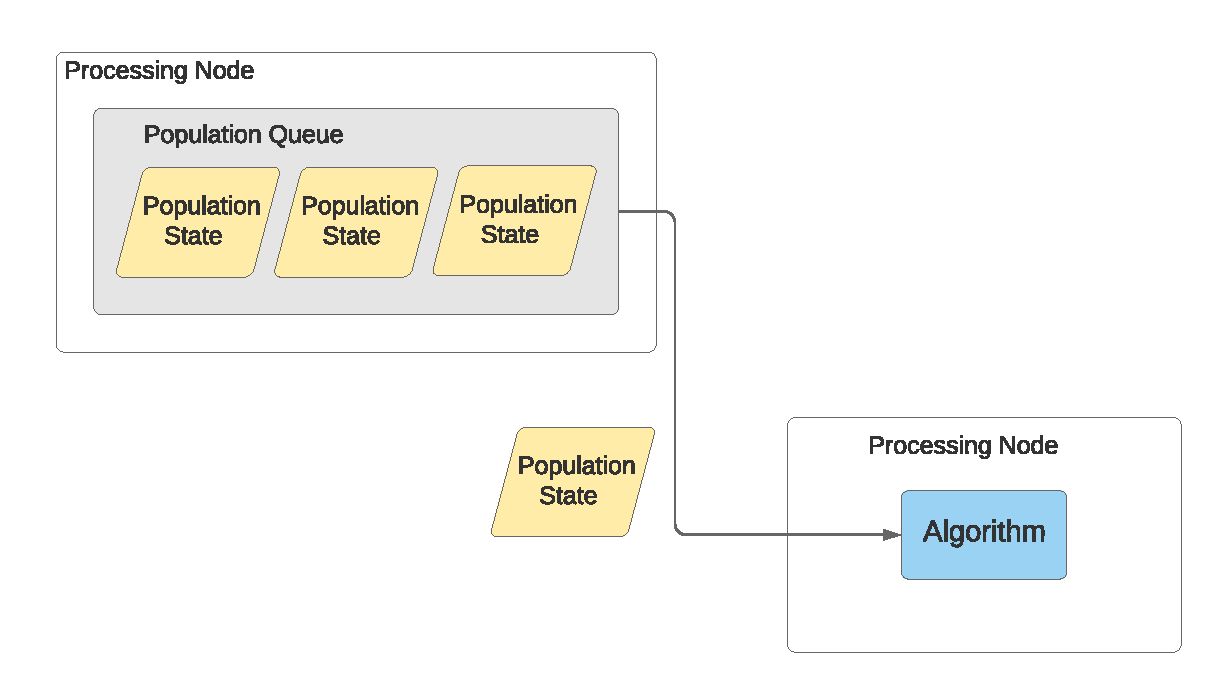
\includegraphics[width=\textwidth]{population_message}
    \caption{Population State and dataflow between processing nodes of a message-based algorithm.}
    \label{fig:population_message}
\end{figure}

On the other hand, there are several caveats as well:
It is more costly to move entire subpopulations as messages than only passing certain individuals 
from a process to another. Designers must conmsider this cost when working with large
individuals, and if possible send sub-populations using several messages, use compression or 
adjust the size of subpopulations. Pool-based algorithms also suffer from this drawback, but 
web based immplementations have been working with continous optimization problems of 1000 dimensions.
But, in other cases this is not a viable approach. 

\begin{figure}[ht]
    \centering
    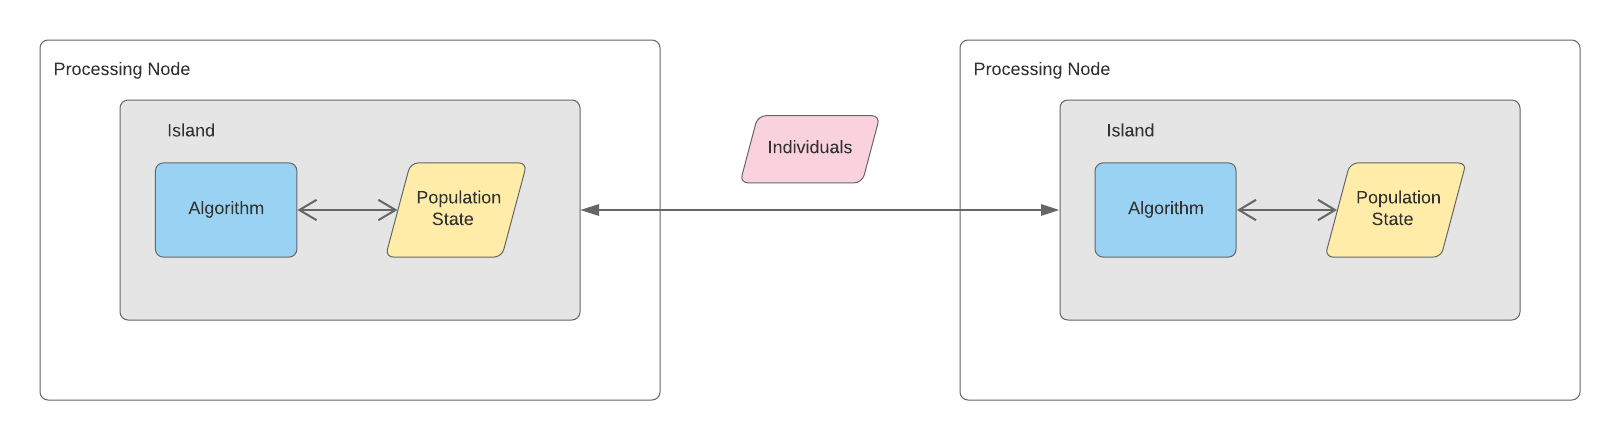
\includegraphics[width=\textwidth]{classicisland}
    \caption{ Population State and dataflow between processing nodes of a classic Island-based multi-population algorithm. }
    \label{fig:classicisland}
\end{figure}

\subsection{Comparison with other cloud-based works} 
\label{comparison}

Next, we compare the message-driven architecture we presented against four other
proposals for multi-population algorithms found in the literature. We center the
comparison on the coupling and communication between the main components:
Subpopulations, Processing Nodes, and Algorithms.  In Figure \ref{fig:population_message} we show the
main components of a message-driven architecture. We can see that the algorithm
and the subpopulations are separated, and the Population Queue keeps the state
of subpopulations. While algorithms only need the subpopulations as parameters
for their execution.

% We need to add references to the respective papers - Mario

In contrast, in the classic Island model shown in Figure
\ref{fig:classicisland}, algorithms are coupled with a subpopulation, and the same processing
node keeps both the algorithm process and the state of the subpopulation.  Other
processing nodes follow the same configuration and form of execution, and they
only pass specific individuals between them.  In this model, adding additional
processing nodes, on-runtime, can be more difficult, because they need to have
an addressing mechanism. % JJ, help I don't know if this is clearly understood, a mean like a DNS - Mario

\begin{figure}[ht]
    \centering
    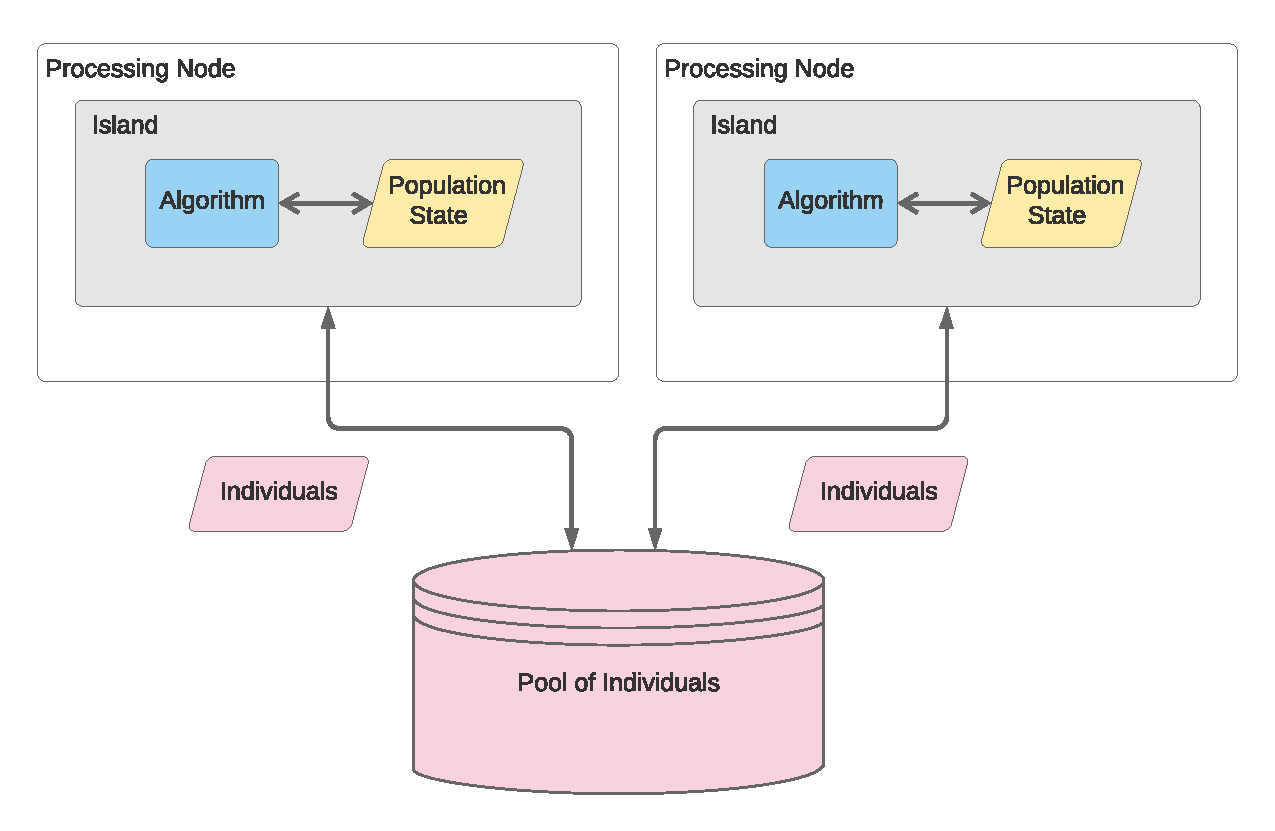
\includegraphics[width=\textwidth]{pool_island}
    \caption{Population State and dataflow between processing nodes of a Pool-based multi-population algorithm.}
    \label{fig:pool_island}
\end{figure}

A typical design pattern used to alleviate the above drawbacks is the use of a
central repository or pool of individuals that is available to all processing
nodes.  In Figure \ref{fig:pool_island} we show the main components of a pool-based
multi-population algorithm. Although algorithms and subpopulation state remains
coupled, now, processing nodes do not communicate directly with each other.
Instead, they interchange individuals with the pool. Communication between nodes
is not affected if the system adds or removes nodes because they do not know
about each other.  Since the state of the global population is stored in
external processing nodes, the system needs additional communication and
processing for keeping track of each subpopulation.

We show another pool-based approach in Figure  \ref{fig:population_pool}. In
this design, the global population is stored in a central repository, while
isolated algorithms take random samples of the global population and use this
temporal subpopulation as parameters. An advantage of this design is that the
sampling provides a type of migration between isolated subpopulations. A problem
found is that when a processing node returns a subpopulation to the pool, the
state of the subpopulation is lost. But having the algorithm decoupled opens the
possibility of having a serverless-function implementation.   

\begin{figure}[ht]
    \centering
    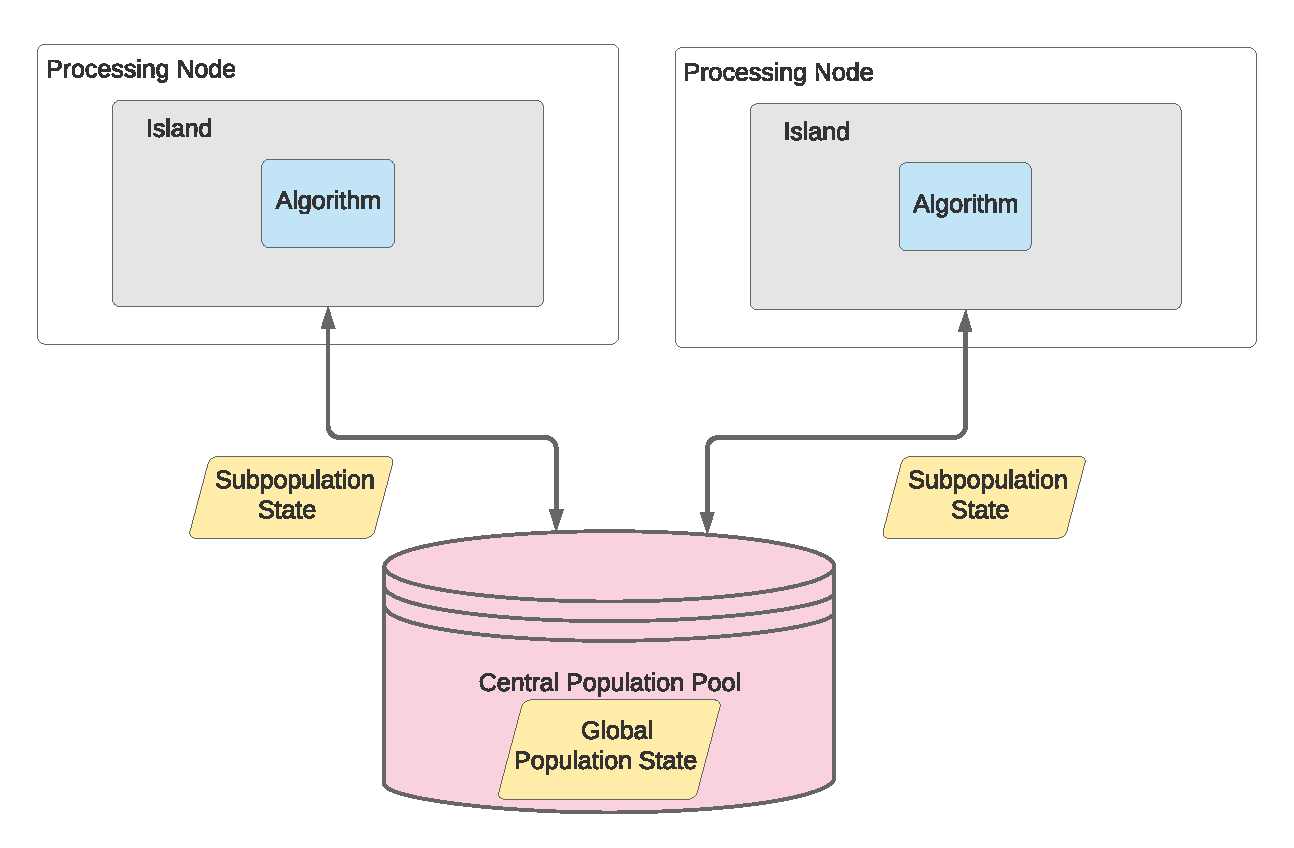
\includegraphics[width=\textwidth]{population_pool}
    \caption{Population State and dataflow between processing nodes of the EvoSpace algorithm.}
    \label{fig:population_pool}
\end{figure}

\section{Container-based application} 
\label{docker}

We have mentioned several advantages of a cloud-native application for running
multi-population based algorithms, but there are in our experience several
practical issues of this approach. In general, cloud platforms have free-tiers
for their services, and many offer academic discounts to students. But once we
pass to the pay-as-you-go tier, computing resources need to be
managed, and, where possible, its cost minimized.  First,
in many cases,  a credit-card is needed to guarantee the payment of the
resources consumed and someone responsible for assigning quotas and, more
importantly, special keys for using the cloud's API.  If these keys are
compromised or shared by their holders,  additional costs or administrative
procedures are in order. For those cases when a prototype platform is needed,
for instance, students developing a new algorithm variant or experimenting with
a published work, a container-based platform can be more practical. Container
technology enables researchers the local deployment of all the infrastructure
needed to run the experiments. Later, if needed, the same deployment could be
deployed to the cloud.
% I don't see this line of argument. You can do exactly the same with
% virtual machines instead of containers. Also, you can test a virtual
% infrastructure locally and then only when it's needed deploy it to
% the cloud. If you want to give good reasons for using containers
% instead of virtual machines, there are quite a lot non-economic ones
% - JJ
% OK, I will add an issue - Mario 

In this section, we propose a design of a reactive container-based application
for executing multi-population based optimization experiments.  For the design,
we followed the design patterns highlighted in the previous section, and again
we can go back to Figure \ref{fig:kafkEO} and use it as a guide for explaining
the main components and their interactions. But first, we give a brief
description of the technology we used.

\subsection{Containers} 
\label{containers}
% TO DO

\subsection{Docker Compose} 
\label{compose}
% TO DO
 

% Do we need a description of every container? Wouldn't a general
% description of the containers used be enough? - JJ 
% Ok, I think only workers and the controller need to be described in detail - Mario 

\subsection{Controller Container} 
\label{controller}

The controller is an essential component of the architecture (Figure \ref{fig:kafkEO})
because it is responsible for maintaining the evolutionary loop. It takes newly
evolved populations from the Output Queue, mixes them,   and produces new
messages from the result. At the same time, it must keep track of two conditions
for ending the loop: the number of messages it has received reaches a maximum
value, or the error of the best solution goes below a specific threshold.  Finally, it
must filter out remnant messages from other experients. Messages from other
experiments can remain in the queues because of the asynchronous nature of the
system.  We chose to implement the controller in Python but using an API
specialized in asynchronous event-driven programming over data streams.  
The open-source library is called Reactive Extensions (ReactiveX) for Python 
\url{https://github.com/ReactiveX/RxPY} an it is based on the Observer 
pattern \cite{gamma1995design} and functional programming.

\begin{figure}[ht]
    \centering
    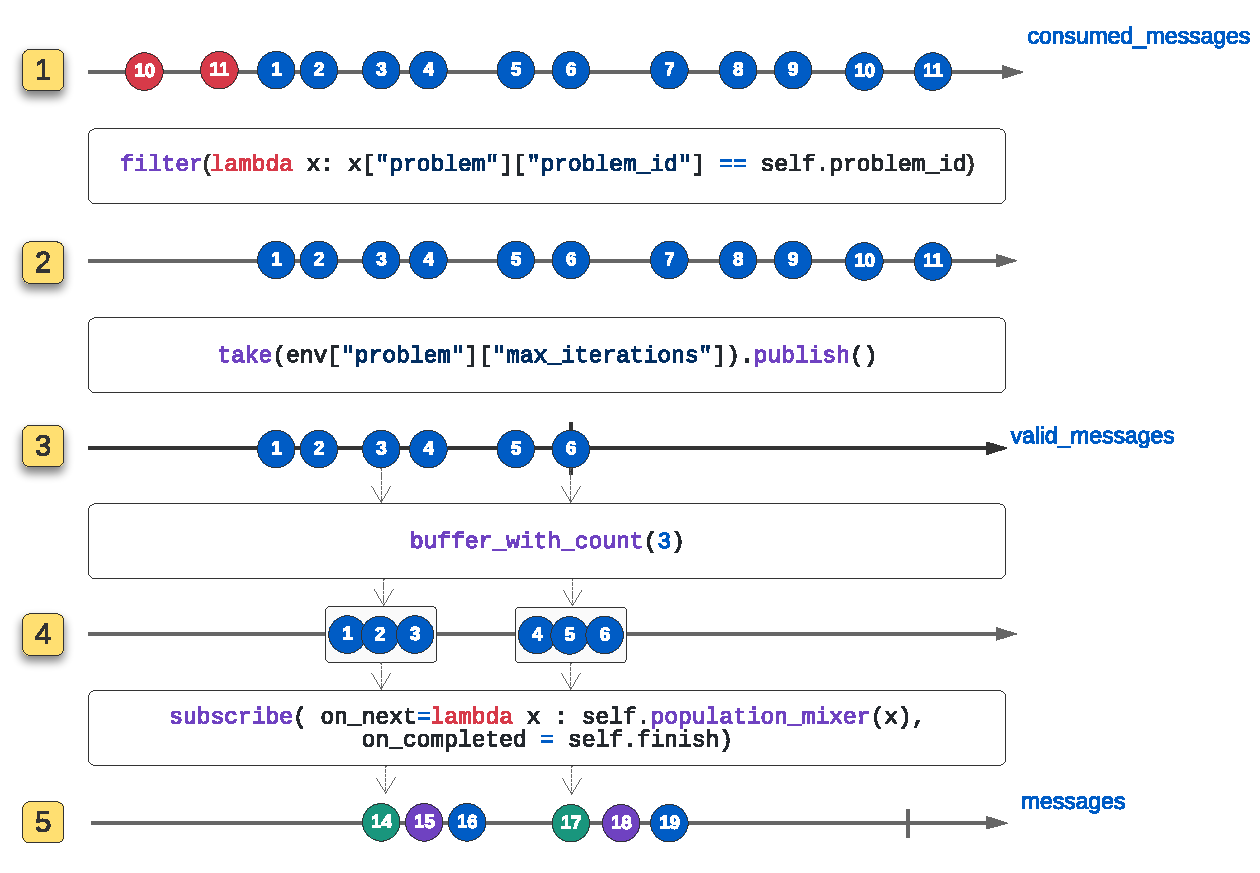
\includegraphics[width=\textwidth]{marble_controller}
    \caption{Marble diagram for the Reactive Python implementation of the Controller}
    \label{fig:marble_controller}
\end{figure}

In ReactiveX, an observer object subscribes to an Observable. Observables emit a
sequence of items, and all the subscribed observers react to each emission. The
ReactiveX library includes several reactive operators that we can use to
transform and combine sequences of items. These operators provide reactive
extensions that allow us to compose asynchronous sequences together in a
declarative manner. In Figure \ref{fig:marble_controller}, we use a so-called marble diagram to
represent the composition of Observables and reactive extensions operators. We
represent the timeline of an Observable as a horizontal arrow, which indicates
that time flows from left to right. In the diagram, items are represented as
marbles. The position of each marble indicates the point in time when they were
emitted by the Observable. Reactive operators are represented as text boxes,
showing the transformation to be applied. Normally, a transformation results in
another Observable, again emitting new results.  For asynchronous programming, 
this approach is more elegant than nested callbacks, that are more difficult 
to code and debug. 

Now we proceed to explain the reactive implementation of the controller.
In Figure \ref{fig:marble_controller}, we  have the following composition of Observables:

\begin{enumerate}

\item The controller continually pulls new messages from the Output 
message queue. These messages are instantly emitted by the  \texttt{consumed\_messages}
Observable. In this particular period, we can see that the stream receives 
two populations from another experiment, and are shown as two red marbles.  
The filter operator removes all messages that belong to a different experiment; 
in this case, we are only interested in blue marbles. 

\item The \texttt{max\_iterations} parameter indicates the number of populations that
are going to be accepted. When this number of messages is reached, we must
end the loop. In this example, \texttt{max\_iterations = 6},  the take operator 
assures that only 6 messages are received. After the Observable emits 
the sixth message, it triggers the completed event.

\item Many observers can be subscribed to the \texttt{valid\_messages}  Observable because it
emits all the valid items. At the moment, there are to additional methods
subscribed that we are not showing, one for logging and the other for monitoring
the search.

\item The   \texttt{buffer\_with\_count(3)} operator, waits until it receives 
three valid messages to emit a single message that contains a list with
the previous three. The migration method requires that list to mix them. 
In our previous work, we needed a local buffer for storing a certain 
number of populations to mix them with others. This design has the advantage
of not needing extra memory, and it integrates better with the reactive paradigm.
A possible disadvantage can be that it only mixes contiguous populations,
but this can be mitigated with a larger buffer.

\item The  \texttt{population\_mixer} method pushes new populations to the messages Observable,
a  \texttt{publish(population)} observer is responsible for pushing 
the newly generated populations back to the Input Message Queue.
\end{enumerate}



\begin{figure}[ht]
    \centering
    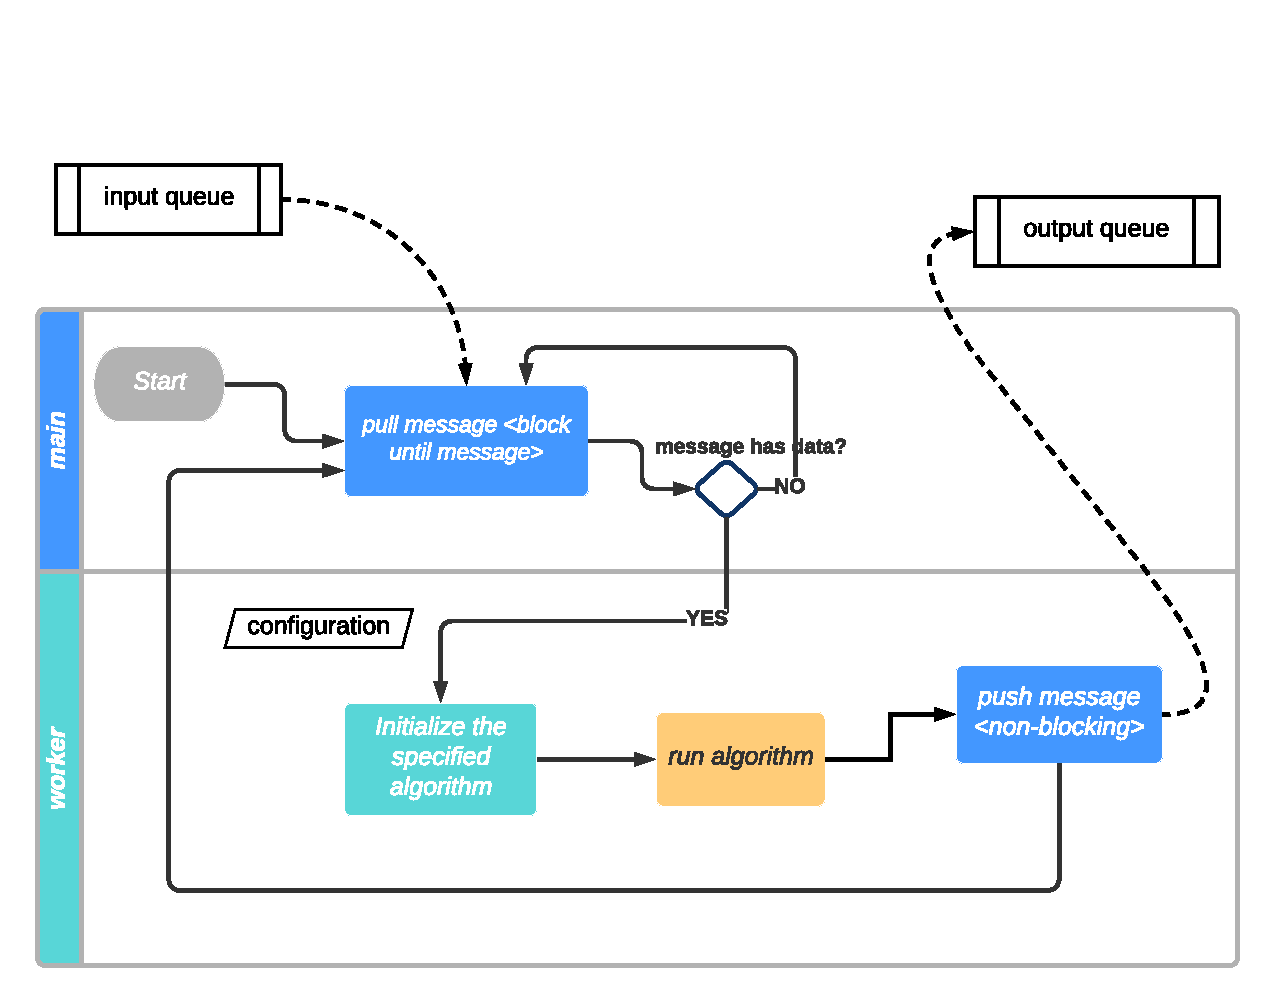
\includegraphics[width=\textwidth]{worker}
    \caption{Serverless function implementation details. Showing the worker algorithm in each container}
    \label{fig:worker}
\end{figure}

\subsection{Worker Containers} 
\label{workers}

Figure \ref{fig:worker}.

\begin{algorithm}
    \caption{Migration}
    \label{read}
    \begin{algorithmic}[1]
        \Procedure{cxBestFromEach}{$pop_1,pop_2$}
            \State $pop_1.sort()$
            \State $pop_2.sort()$
            \State $size\gets min(len(pop_1), len(pop_2))$
            \State $cxpoint\gets (size-1)/2$
            \State $pop_1[cxpoint:]\gets pop_2[:cxpoint+2]$
            \State \textbf{return} $pop_1$
        \EndProcedure
            
    \end{algorithmic}
\end{algorithm}

\subsection{Experimental Process} 
\label{experiment_flow}


\begin{sidewaysfigure}
    \centering
    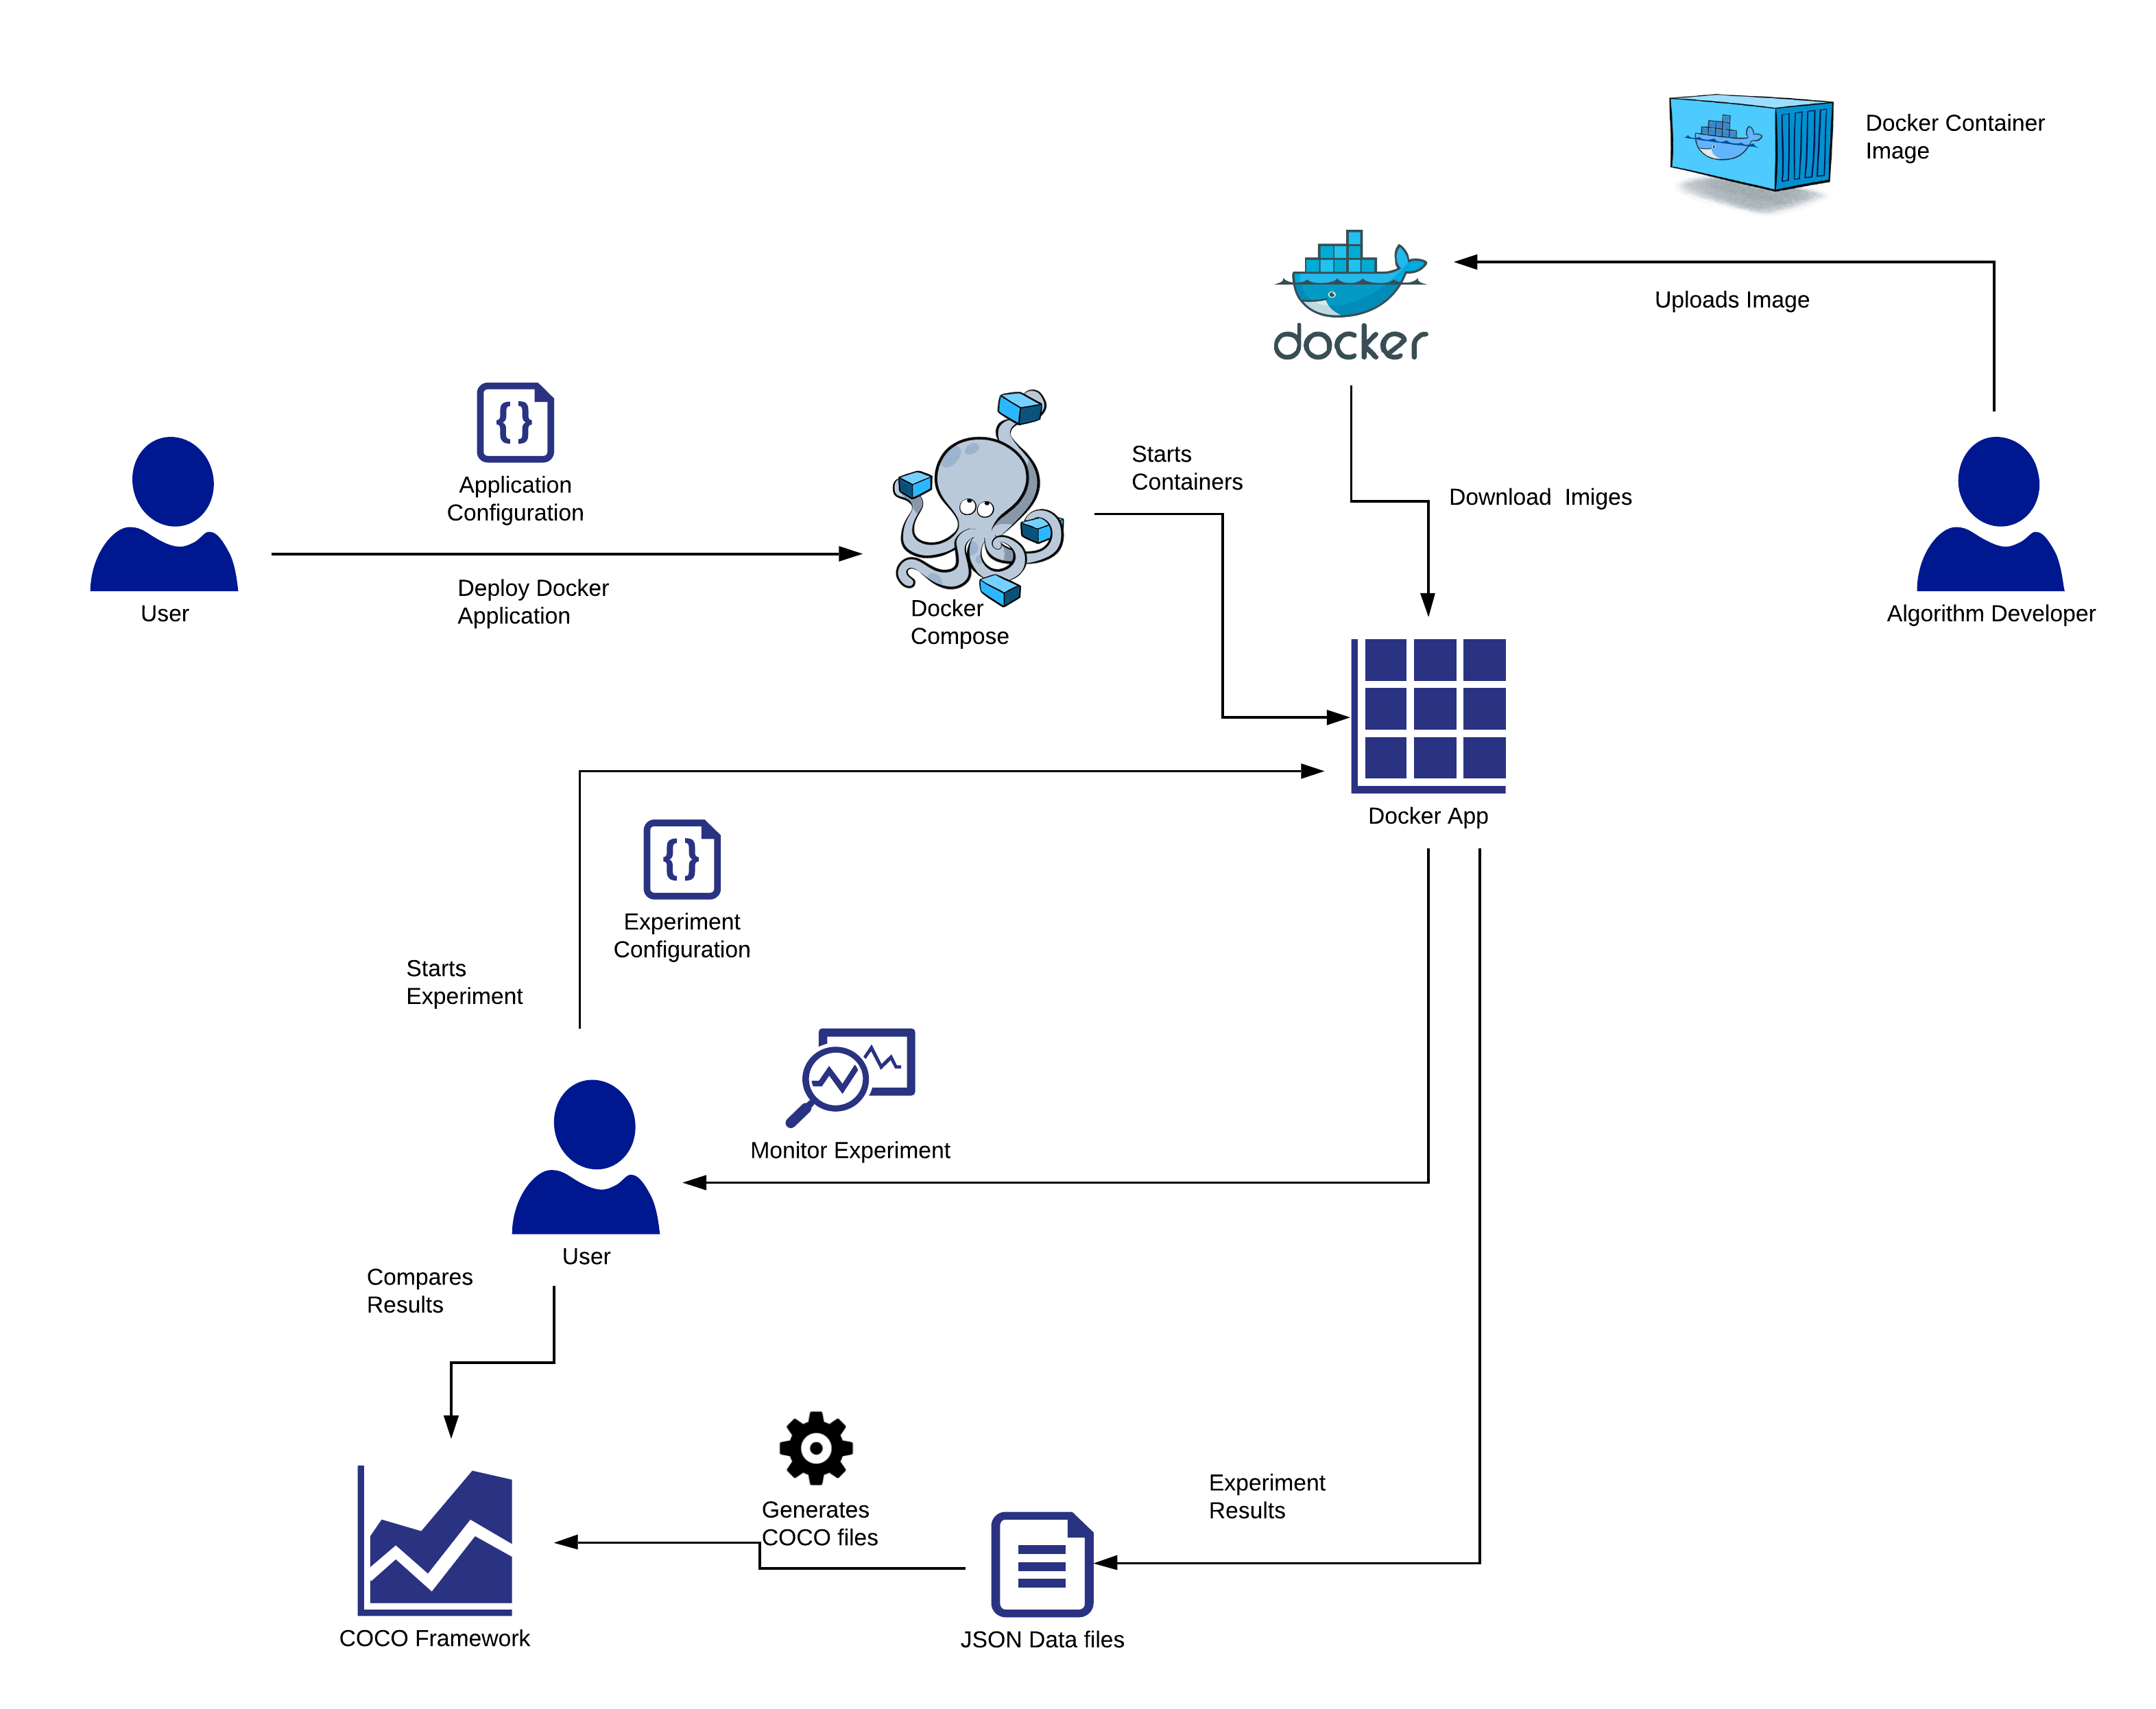
\includegraphics[width=\textwidth]{experiment_flow}
    \caption{EvoSwarm Workflow}
    \label{fig:experiment_flow}
\end{sidewaysfigure}

Figure \ref{fig:experiment_flow} shows the workflow users can follow to run
experiments in Evo\-Swarm. The first step is to develop the search strategy
algorithms that are going to be used by the multi-population algorithm.
Algorithm Developers can upload the container definition or images directly to
DockerHub. Another option is to upload the image definition (Dockerfile) to
GitHub and define a trigger to re-upload the image to DockerHub.  Docker Compose
configuration files can reference these containers. When a user needs to deploy
the application, he or she needs to edit the Docker compose file to specify the
type and number of containers needed for the application.  The Docker compose
application is responsible for starting all the containers or downloading new
versions if it is necessary. After starting the application, users can push
Experiment Definition files and start monitoring the execution in the terminal.
After the experiment is finished, the user must execute another script using the
experiment id to generate a collection of files containing all the data
generated by the experiment. The script generates these files in a JSON format.
Researchers can use these files to analyze and plot experiment data.  Python
scripts are included in the repository to plot the running times for the
experiments, and all other plots used in this paper.  There is also a script to
generate the files needed by the COCO framework \cite{hansen2016coco}, which can generate standard
comparisons against other methods.










\section{Experimental Setup} 
\label{setup}

\section{Experimental Results} 
\label{results}

\begin{figure}[ht]
    \centering
    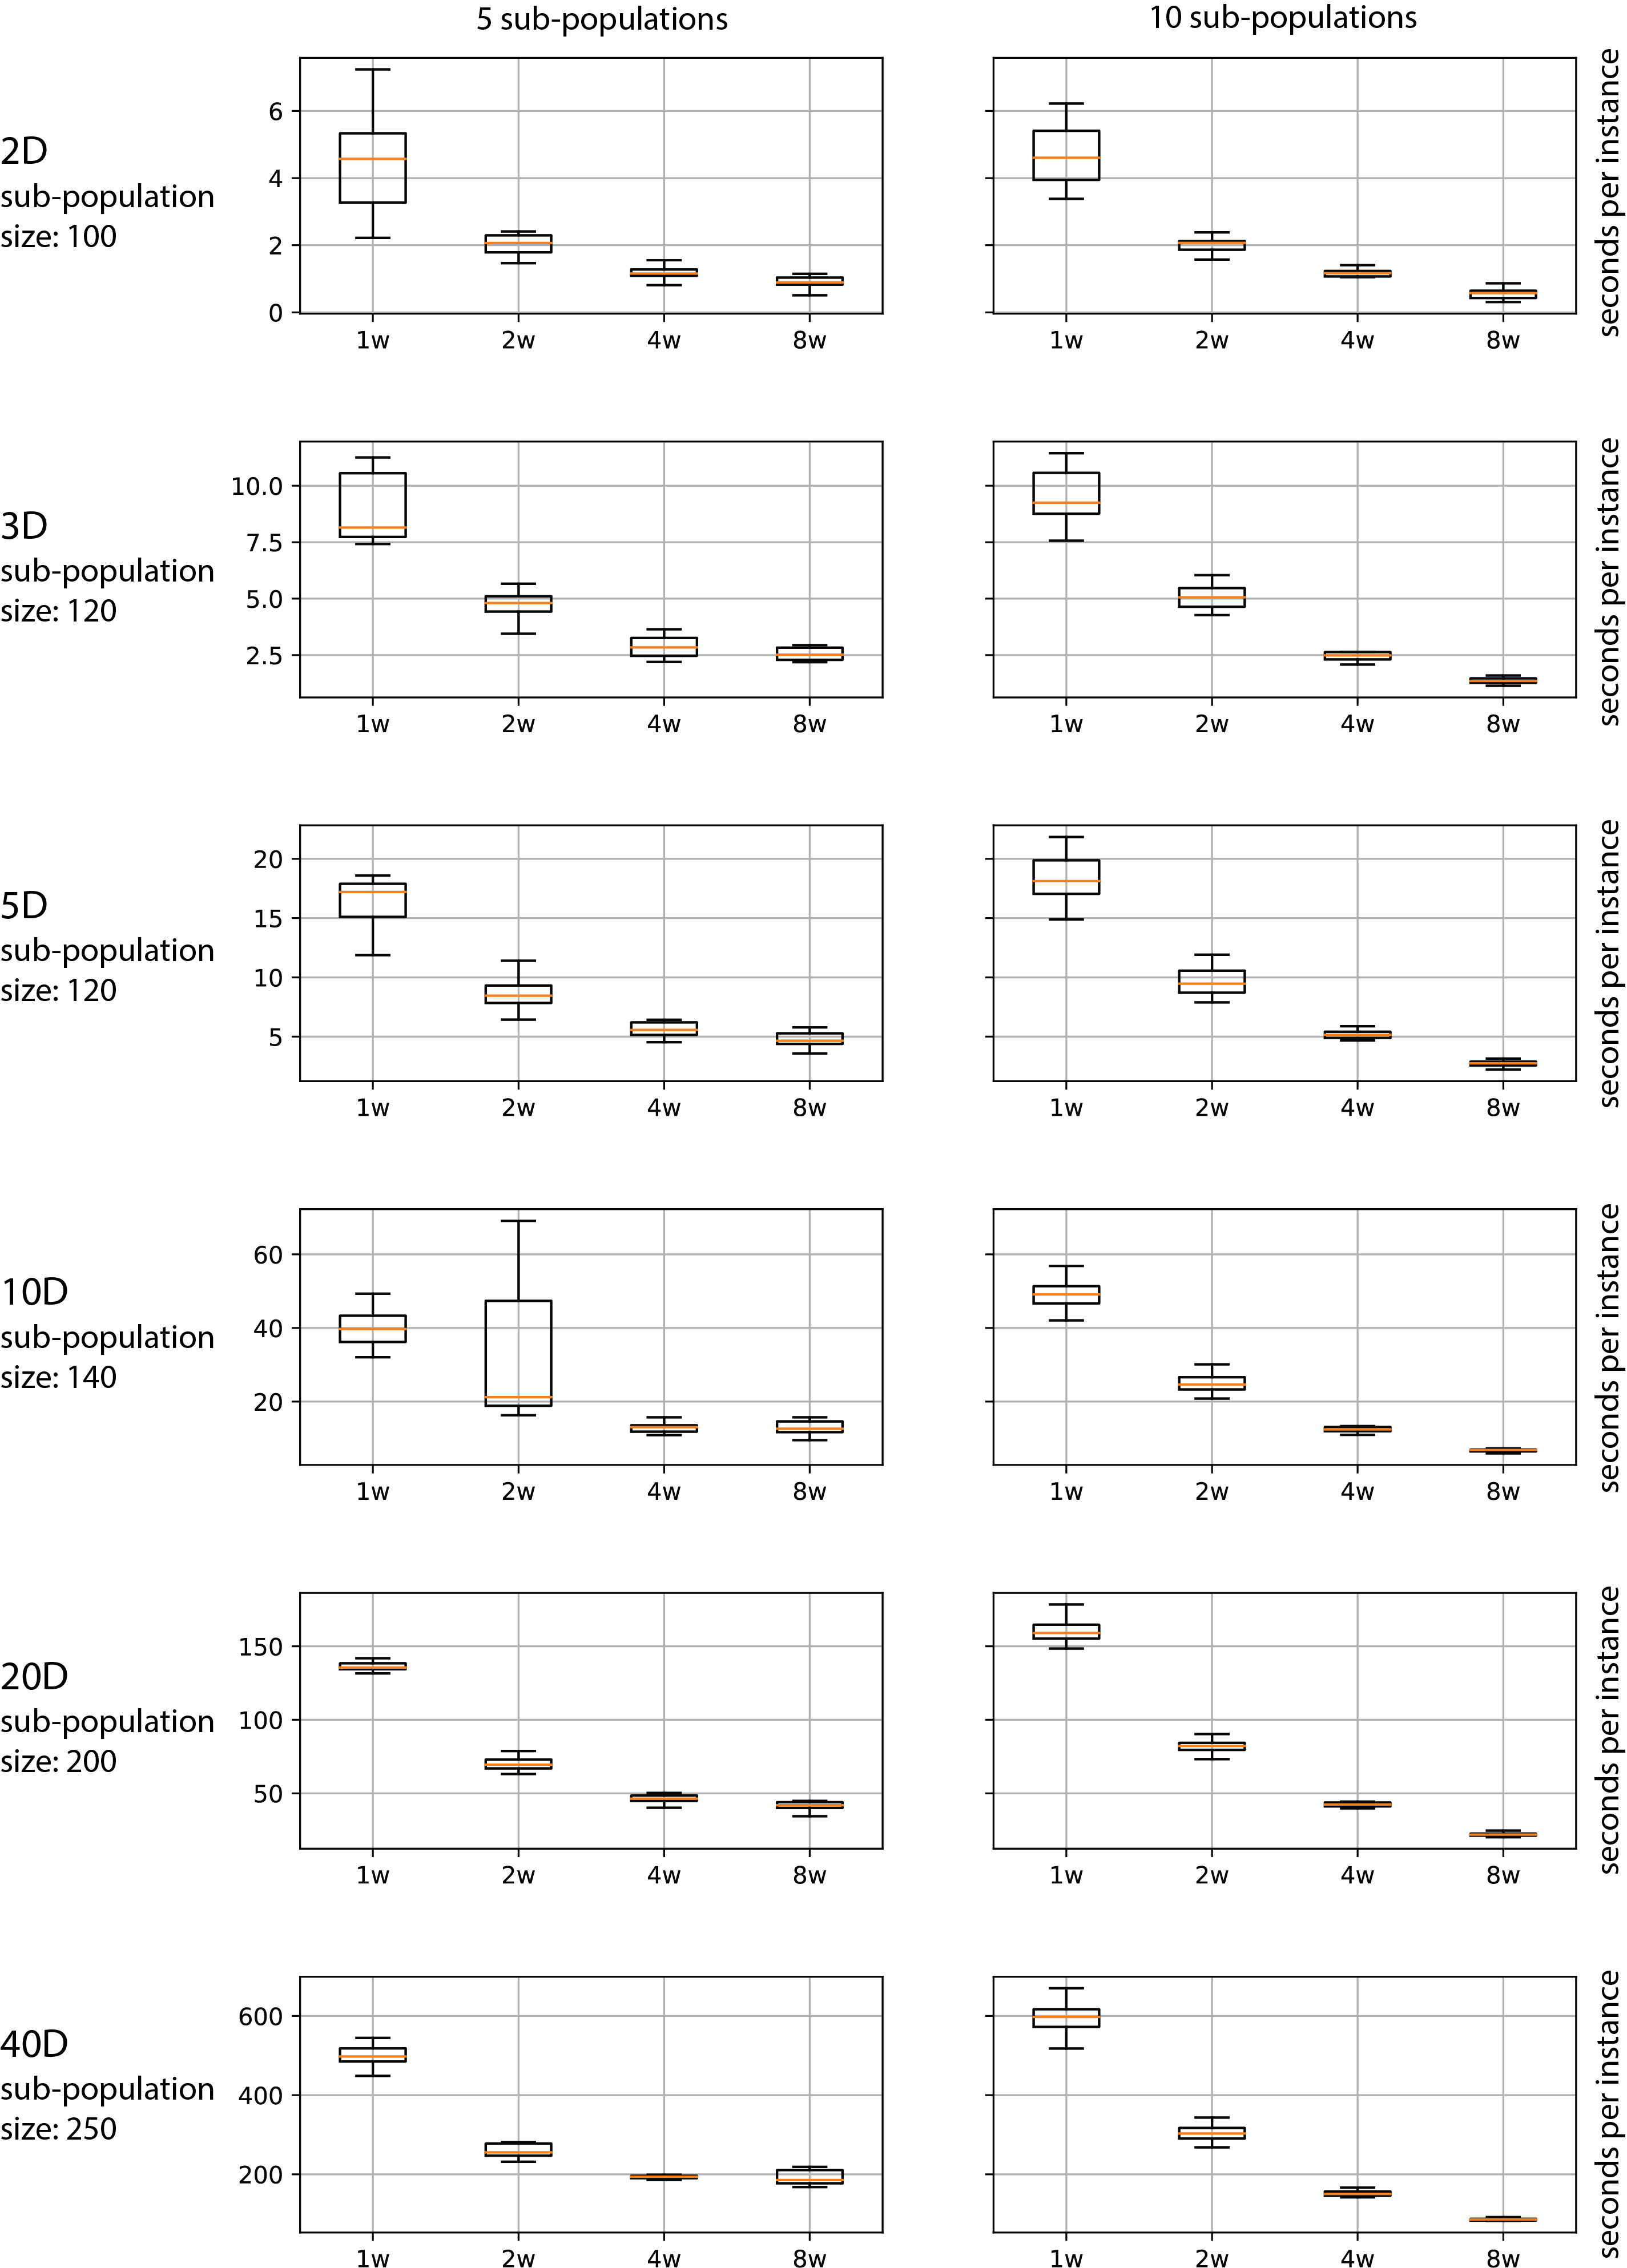
\includegraphics[width=\textwidth]{sp_size_worker}
    \caption{ TO DO}
    \label{fig:worker}
\end{figure}

\section{Conclusions} 
\label{conclusions}

\bibliographystyle{elsarticle-num}
\bibliography{multipopulation}

\end{document}